\newaufgabe{
Implementieren sie (natürlich unter zu-Hilfenahme einer AES realisierenden Library)
ECM und CBC unter AES selbst und bestätigen sie experimentell das beschriebene
Verhalten von CBC bei Ciphertextfehlern. Vergleichen sie weiters ihre ECM und
CBC Varianten mit den Varianten die die Library zur Verfügung stellt bzgl. der
benötigten Rechenzeit.
}
\paragraph{Implementierung}
Die Implementierung der Blockchiffremodi erfolgte in der Programmiersprache Rust. Zu diesem Zweck wurden zwei zentrale Funktionen, \texttt{encrypt} und \texttt{decrypt}, erstellt, die jeweils den gewünschten Modus als Parameter erhalten.
Die \texttt{decrypt}-Funktion ist analog aufgebaut. 
\begin{minted}{rust}
pub fn encrypt<T: AsRef<[u8]>>(
        msg: T, 
        key: &[u8; 16], 
        mode: BlockCipherMode
    ) -> Vec<u8> {
    // ...
    match mode {
        BlockCipherMode::ECM => 
            ecm::encrypt(msg, Aes128::new(key)),
        BlockCipherMode::CBC(iv) => 
            cbc::encrypt(msg, Aes128::new(key), iv)
        _ => msg,
    }
}
\end{minted}
\paragraph{ECM}
Im ECM wird der Klartext in Blöcke zu jeweils 16 Byte (128 Bit) aufgeteilt. Jeder Block wird unabhängig von den anderen verschlüsselt.
\begin{minted}{rust}
// ECM MODE
pub fn encrypt(mut msg: Vec<u8>, cipher: Aes128) -> Vec<u8> {
    msg.chunks_exact_mut(16)
        .map(GenericArray::from_mut_slice)
        .for_each(|block| cipher.encrypt_block(block));
    msg
}

pub fn decrypt(mut msg: Vec<u8>, cipher: Aes128) -> Vec<u8> {
    msg.chunks_exact_mut(16)
        .map(GenericArray::from_mut_slice)
        .for_each(|block| cipher.decrypt_block(block));
    msg
\end{minted}
\paragraph{CBC-Modus}
Im CBC-Modus (Cipher Block Chaining) wird zusätzlich der vorherige Chiffretextblock mit dem aktuellen Klartextblock per XOR verknüpft, bevor die Verschlüsselung erfolgt. Für den ersten Block wird dabei ein Initialisierungsvektor (IV) verwendet.
\begin{minted}{rust}
// CBC MODE
pub fn encrypt(mut msg: Vec<u8>, cipher: Aes128, iv: [u8; 16]) -> Vec<u8> {
    let mut prev = &GenericArray::from(iv);
    for block in msg
        .chunks_exact_mut(16)
        .map(GenericArray::<u8, U16>::from_mut_slice)
    {
        block.iter_mut().zip(prev).for_each(|(a, &b)| *a ^= b);
        cipher.encrypt_block(block);
        prev = block;
    }
    msg
}
\end{minted}
Die Entschlüsselung erfolgt in umgekehrter Reihenfolge. Ein \texttt{Peekable}-Iterator ermöglicht während der Iteration den Zugriff auf den nachfolgenden Block mithilfe von \texttt{peek()}. Ist kein weiterer Block vorhanden, wird der Initialisierungsvektor verwendet.
\begin{minted}{rust}
pub fn decrypt(mut msg: Vec<u8>, cipher: Aes128, iv: [u8; 16]) -> Vec<u8> {
    let mut block_iter = msg
        .chunks_exact_mut(16)
        .map(GenericArray::<u8, U16>::from_mut_slice)
        .rev()
        .peekable();

    while let Some(block) = block_iter.next() {
        let prev = match block_iter.peek() {
            Some(b) => b,
            None => &GenericArray::from(iv),
        };

        cipher.decrypt_block(block);
        block.iter_mut().zip(prev).for_each(|(a, &b)| *a ^= b);
    }

    msg
}
\end{minted} 
\paragraph{Verhalten bei Bitfehlern}
Zur Veranschaulichung des Fehlerfortpflanzung wurden quadratische, einfarbige Bilder verschlüsselt und anschließend wieder entschlüsselt. Dabei wurden sowohl der ECB- als auch der CBC-Modus verwendet.
\begin{table}
    \begin{center}
        \begin{tabular}{|c|c|c|c|}
        \hline
        Modus & Klartext & Chiffretext & Entschlüsselung \\
        \hline
        ECB &
        
\includegraphics[width=3cm]{img/no_error/original} &
        
\includegraphics[width=3cm]{img/no_error/output_ECM} &
        
\includegraphics[width=3cm]{img/no_error/output_ECM_decrypt} \\
        \hline
        CBC &
        
\includegraphics[width=3cm]{img/no_error/original} &
        
\includegraphics[width=3cm]{img/no_error/output_CBC} &
        
\includegraphics[width=3cm]{img/no_error/output_CBC_decrypt} \\
        \hline
        \end{tabular}   
    \end{center}
    \caption{Verschlüsselung und Entschlüsselung ohne Bitfehler}
\end{table}
Wird ein Bit im Chiffretext verändert, so zeigen sich beim ECB-Modus nur lokale Veränderungen im entsprechenden Block. Im CBC-Modus hingegen beeinflusst ein einzelner Bitfehler nicht nur den fehlerhaften Block selbst, 
sondern auch ein Bit im darauffolgenden. Das entspricht der erwarteten 
Fehlerfortpflanzung (siehe. Tabelle \ref{tab:biterror}, klein im linken unteren Eck).
\begin{table}
    \begin{center}
        \begin{tabular}{|c|c|c|c|}
        \hline
        Modus & Klartext & Chiffretext & Entschlüsselung \\
        \hline
        ECB &
        
\includegraphics[width=3cm]{img/error/original} &
        
\includegraphics[width=3cm]{img/error/output_ECM} &
        
\includegraphics[width=3cm]{img/error/output_ECM_decrypt} \\
        \hline
        CBC &
        
\includegraphics[width=3cm]{img/error/original} &
        
\includegraphics[width=3cm]{img/error/output_CBC} &
        
\includegraphics[width=3cm]{img/error/output_CBC_decrypt} \\
        \hline
        \end{tabular}   
    \end{center}
    \caption{Verschlüsselung und Entschlüsselung mit Bitfehler}
    \label{tab:biterror}
\end{table}
\newpage
\paragraph{Benchmarking}
Die Ausführungsgeschwindigkeit der selbst implementierten Modi wurde in einem Benchmark mit der Referenzimplementierung der verwendeten Bibliothek verglichen.
\begin{figure}[h]
    \centering
    \begin{subfigure}[b]{0.49\textwidth}
        \centering
        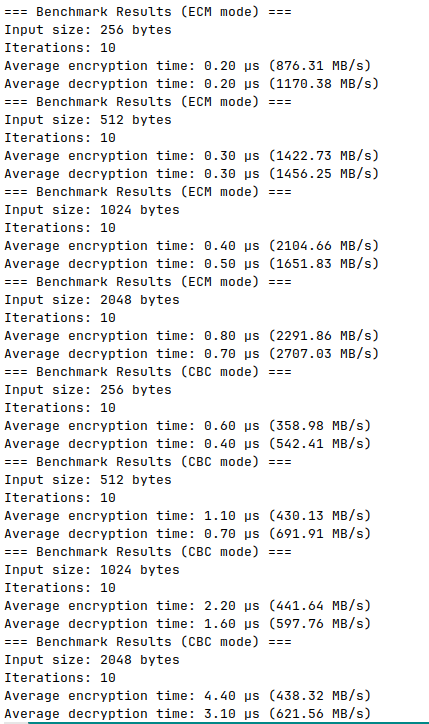
\includegraphics[width=\textwidth]{img/bench/custombench}
        \caption{Eigene Implementierung}
        \label{fig:bench_my}
    \end{subfigure}
    \hfill
    \begin{subfigure}[b]{0.49\textwidth}
        \centering
        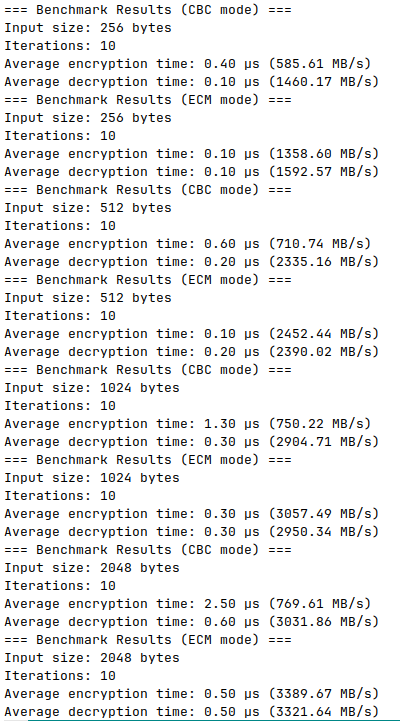
\includegraphics[width=\textwidth]{img/bench/referencebench.png}
        \caption{Referenzimplementierung}
        \label{fig:bench_ref}
    \end{subfigure}
    \caption{Vergleich der Ausführungszeiten}
    \label{fig:benchmark}
\end{figure}
Die Ergebnisse zeigen, dass die eigene Implementierung bei kleineren Datenmengen vergleichbare Laufzeiten wie die Referenz erreicht. Bei größeren Klartexten nimmt die Performanz jedoch merklich ab, während die Referenzimplementierung eine konstantere Ausführungsgeschwindigkeit beibehält.